---
id: tkz-euclide-ejemplo-52
title: "Ángulo agudo"
description: "Creación de un ángulo agudo"
keywords: [angulo,agudo,rayo,taller1]
tags: [tkzDefShiftPoint,tkzFillAngle,tkzMarkAngle,tkzDrawLines]
sort: 52
---
\documentclass[tikz,border=2mm]{standalone}
\usepackage{tkz-base}
\usepackage{tkz-euclide}

\begin{document}
    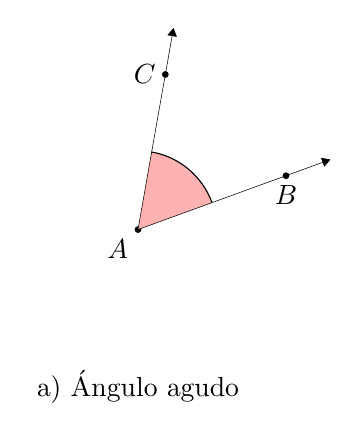
\begin{tikzpicture}
        % Paso 1: Define vértice del ángulo
        \tkzDefPoint(1,2){A}

        % Paso 2: Define punto del rayo inferior
        \tkzDefPoint(3,2){B}
        
        % Paso 3: Encuentra un punto C a 20°            
        \tkzDefShiftPoint[A](20:2){B}
        
        % Paso 4: Encuentra un punto C a 80°            
        \tkzDefShiftPoint[A](80:2){C}

        % Paso 5: Dibuja los puntos y etiquétalos
        \tkzDrawPoints(A,B,C)
        \tkzLabelPoints[below left](A)
        \tkzLabelPoints[below](B)
        \tkzLabelPoints[left](C)

        % Paso 6: Marca y rellena el ángulo
        \tkzFillAngle[fill=red!30](B,A,C) % ∠BAC
        \tkzMarkAngle(B,A,C)              % ∠BAC

        % Paso 7: Dibuja los segmentos de los rayos
        \tkzDrawLines[add=0 and 0.3, -Triangle](A,C A,B)

        % Paso 8: Agrega leyenda al gráfico
        \tkzText(1,0){a) Ángulo agudo}                
    \end{tikzpicture}
\end{document}
